% SPDX-License-Identifier: CC-BY-4.0
% Copyright (c) 2026 Alexander Stephen Donahue (Independent Researcher, ORCID 0009-0006-8168-9648)
\documentclass[11pt,letterpaper]{amsart}

\usepackage[margin=0.92in]{geometry}
\usepackage{amsmath,amssymb,amsthm}
\usepackage{graphicx}
\usepackage{booktabs}
\usepackage{array}
\usepackage{tabularx}
\usepackage{xcolor}
\usepackage{xurl}
\usepackage{hyperref}
\usepackage{microtype}
\emergencystretch=3em
\raggedbottom
\newcolumntype{L}{>{\raggedright\arraybackslash}X}

\hypersetup{
  colorlinks=true,
  linkcolor=blue!65!black,
  citecolor=blue!65!black,
  urlcolor=blue!65!black,
  pdftitle={A Formally Verified, Multi-Scale Computational Framework for the Human Synaptic Bouton},
  pdfauthor={Alexander Stephen Donahue}
}

\newtheorem{theorem}{Theorem}[section]
\newtheorem{proposition}[theorem]{Proposition}
\newtheorem{remark}[theorem]{Remark}

\title[Formally Verified Human Synaptic Bouton Biophysics]{A Formally Verified, Multi-Scale Computational Framework for the Human Synaptic Bouton: Exact Biophysics, Stochastic Nanocolumn Coupling, Bioenergetics, and DNA-Origami Metrology}

\author{Alexander Stephen Donahue}
\address{Independent Researcher, Spokane, WA, USA}
\email{0\_0@0thernes.art}
\thanks{ORCID: \href{https://orcid.org/0009-0006-8168-9648}{0009-0006-8168-9648}. Zenodo Concept DOI: \href{https://doi.org/10.5281/zenodo.24477927}{10.5281/zenodo.24477927} (all versions; prior v1.3.0 Version DOI \href{https://doi.org/10.5281/zenodo.24548051}{10.5281/zenodo.24548051}). Code and Lean~4 proofs licensed under Apache-2.0; manuscript, figures, blueprint, and datasets licensed under CC-BY-4.0. Repository: \url{https://github.com/0thernes/human-synapse-bouton-lab}. Interactive Lean Blueprint: \url{https://0thernes.github.io/human-synapse-bouton-lab/blueprint/}. Preprint v1.4.0; not externally peer-reviewed.}
\date{November 26, 2026}

\begin{document}

\begin{abstract}
Quantitative electron tomography, native synaptic vesicle cryo-EM, and super-resolution DNA-PAINT/RESI metrology have revealed that the human cortical synaptic bouton is a hyper-crowded ($\sim 300{,}000$-protein baseline in rat synaptosomes, with $2\text{--}3\times$ larger active zones and $4.0\text{--}9.4\times$ larger mean vesicle pools in human temporal neocortical boutons) stochastic biophysical engine rather than an empty textbook compartment. However, computational neuroscience software rarely combines cross-language numerical verification, pre-registered Monte Carlo falsifiability, and machine-checked mathematical proof. We present \texttt{human-synapse-bouton-lab} v1.4.0, a full-stack multi-language framework (Lean~4.35.0, Rust, strict TypeScript, and Python with a 50-digit \texttt{mpmath}/rational reference oracle) covering presynaptic $\mathrm{Ca}^{2+}$ nanodomains, Hill $n=4$ release cooperativity, Tsodyks--Markram short-term plasticity, Nernst/GHK electrochemistry, conductance-based KCC2/NKCC1 shunting inhibition, Jahr--Stevens NMDAR $\mathrm{Mg}^{2+}$ gating, SNAREpin zippering and Synaptotagmin-1/Complexin clamp kinetics, V-ATPase bioenergetics, kinesin-1 axonal logistics, 4D Hodgkin--Huxley RK4 dynamics, and DNA-PAINT/RESI localization metrology. Twenty-four elementary algebraic, inductive, conservation, monotonicity, and $2\times 2$ integer determinant invariants are formally verified in pure Lean~4.35.0 (zero unused hypotheses, zero \texttt{sorry}, zero \texttt{native\_decide}, and strictly enforced zero \texttt{Classical.choice}), validated with 27 concrete non-vacuity witnesses and 7 sanity and sharpness checks (\texttt{AdversarialChecks.lean}), linked directly to the Python, TypeScript, and Rust engines via executable Lean vector export (\texttt{ExportVectors.lean}), and accepted by six independent kernels via \texttt{lake comparator --paranoid} (\texttt{lean}, \texttt{leanchecker-paranoid}, \texttt{lean4lean}, \texttt{nanoda}, \texttt{con-leche}, and \texttt{con-ron}) in repository CI. Cross-language differential testing verifies agreement within $10^{-10}$ relative error across $1{,}000$ seeded random inputs between TypeScript, Rust, and our 50-digit Python oracle. Finally, we report a pre-registered 30-seed Monte Carlo experiment (Holm--Bonferroni adjusted, 10,000-resample 95\% bootstrap CIs): trans-synaptic nanocolumn alignment ($0$ vs.\ $80\,$nm, $p_{\mathrm{Holm}}=0.0005$, Cliff's $\delta=+1.00$) and tight $\mathrm{Ca}^{2+}$ coupling ($17$ vs.\ $60\,$nm, $p_{\mathrm{Holm}}=0.0005$, $\delta=+1.00$) are strongly confirmed in simulation, a disjoint-seed null control passes ($p_{\mathrm{Holm}}=0.9963$), and our pre-registered 40\,Hz bioenergetic prediction (H3) \emph{fails in simulation} ($p_{\mathrm{Holm}}=1.0000$) because 40\,Hz exceeds the illustrative model's mitochondrial critical frequency ($29.5625\,$Hz), with an upper bound guaranteeing depletion by $t \ge 3\,$s machine-proved in Lean~4.35.0 alongside a transparently logged post-hoc 20\,Hz exploratory follow-up (H3b).
\end{abstract}

\maketitle

\section{Introduction and Claims Ledger}

Between 2000 and 2026, quantitative proteomics \cite{wilhelm2014composition}, human temporal-lobe biopsy 3D electron microscopy \cite{yakoubi2019layer4,rollenhagen2020human,rollenhagen2024l1}, the 1.4-petabyte Harvard--Google H01 human cortical connectome \cite{shapsoncoe2024h01}, native synaptic vesicle cryo-EM of V-ATPase in rat brain \cite{coupland2024vatpase} and the V-ATPase--synaptophysin complex in mouse \cite{wang2024vatpase}, near-atomic microtubule--tau structural maps \cite{kellogg2018tau}, lysosomal RNA-granule hitchhiking via Annexin~A11 and BORC \cite{liao2019anxa11,depace2024borc}, synapsin liquid--liquid phase separation \cite{milovanovic2018llps}, and \AA{}ngstr\"om-scale RESI/DNA-PAINT microscopy \cite{reinhardt2023resi} transformed synaptic neurobiology into a precision nanoscale physical science.

To prevent silent numerical bugs, unverified prose claims, and species-parameter conflation, every quantitative claim in this paper is indexed in Table~\ref{tab:claims} with an explicit epistemic tag: \texttt{kernel-checked} (Lean~4.35.0), \texttt{exact-oracle} (50-digit \texttt{mpmath} / exact rational), \texttt{numerical\_approx.} (float64 ODE or Monte Carlo), \texttt{refuted-prereg.}, or \texttt{empirical-literature}.

\begin{table}[htbp]
\centering
\caption{Numbered Claims Ledger with Epistemic Tags and Verification Outcomes (v1.4.0).}
\label{tab:claims}
\footnotesize
\begin{tabularx}{\textwidth}{@{}l>{\raggedright\arraybackslash}p{4.95cm}>{\raggedright\arraybackslash}p{2.95cm}L@{}}
\toprule
\textbf{ID} & \textbf{Claim} & \textbf{Epistemic Tag} & \textbf{Verification / Outcome} \\
\midrule
C01 & 24 elementary biophysical \& $2\times 2$ determinant lemmas hold with 0 unused hypotheses, 0 \texttt{sorry}, and enforced 0 \texttt{Classical.choice}. & \texttt{kernel-checked} & Lean~4.35.0 + 27 witnesses + 7 sanity/sharpness checks across 6 CI kernels + \texttt{ExportVectors.lean} parity. \\
C02 & TypeScript, Rust, and 50-digit Python oracle agree within $10^{-10}$ across 1,000 random inputs and exported Lean vectors. & \texttt{exact-oracle} & \texttt{test\_differential.py} (2,000 cross-checks + Lean vector bridge, 0 mismatches, NaN/Inf guarded). \\
C03 & H1 (Pre-reg.\ sim.): Aligned ($0\,$nm) nanocolumn yields higher $|\text{EPSC}|$ than $80\,$nm offset across 30 seeds. & \texttt{numerical\_approx.} & Confirmed in sim.: $33.81$ vs.\ $12.28\,$pA, $\delta=+1.00$, $p_{\mathrm{Holm}}=0.0005$. \\
C04 & H2 (Pre-reg.\ sim.): $17\,$nm $\mathrm{Ca}^{2+}$ nanodomain yields higher $\hat{P}_r$ than $60\,$nm microdomain across 30 seeds. & \texttt{numerical\_approx.} & Confirmed in sim.: $0.569$ vs.\ $0.0007$, $\delta=+1.00$, $p_{\mathrm{Holm}}=0.0005$. \\
C05 & H3 (Pre-reg.\ sim.): Under illustrative model constants, mitochondria sustain $>90\%$ ATP at 40\,Hz over 60\,s vs.\ glycolysis $<50\%$. & \texttt{refuted-prereg.} & \textbf{Failed in sim.}: both arms hit $0.0$ ($p_{\mathrm{Holm}}=1.0$); 40\,Hz $> 29.56\,$Hz (T15 upper bound: $0$ by $t\ge 3\,$s). \\
C06 & H4 (Pre-reg.\ Null): Disjoint seed blocks (1000--1029 vs.\ 2000--2029) show no spurious difference. & \texttt{numerical\_approx.} & Passed null: $\Delta=+0.024\,$pA, 95\% CI $[-0.045,+0.091]$, $p_{\mathrm{Holm}}=0.9963$. \\
C07 & H3b (Post-hoc exploratory sim.\ at 20\,Hz): Under illustrative constants, mitochondria sustain $100\%$ ATP while glycolysis hits $0\%$. & \texttt{numerical\_approx.} & Logged in \texttt{DEVIATIONS.md}: $1.00$ vs.\ $0.00$, $\delta=+1.00$, $p_{\mathrm{Holm}}=0.0005$ (fixed-parameter model property). \\
C08 & Rust \texttt{synapse-sim} outperforms Node on 5,000 stochastic APs ($\times 10$ runs + 3 warmups). & \texttt{numerical\_approx.} & Rust median $0.3093\,$ms (IQR $0.0126$) vs.\ clean JSON Node bench (\texttt{data/benchmarks/}). \\
\bottomrule
\end{tabularx}
\end{table}

\section{Human Synaptic Bouton Architecture and Species Scaling}

A recurring defect in earlier computational prototypes (audited as Finding \texttt{F03}) was labeling a bouton with $N=374$ total vesicles (from rat synaptosome proteomics \cite{wilhelm2014composition}) as a human cortical bouton. Quantitative 3D electron microscopy of human temporal-lobe neocortex biopsies demonstrates roughly $2\text{--}3\times$ larger active zones and (author-computed ratios relative to the 374-vesicle rat synaptosome baseline) $4.0\text{--}9.4\times$ larger mean vesicle pools: human Layer~1 boutons average $\sim 3{,}500$ vesicles ($\sim 0.20\,\mu\mathrm{m}^2$ active zone) \cite{rollenhagen2024l1}, Layer~4 averages $\sim 1{,}800$ vesicles ($\sim 0.13\,\mu\mathrm{m}^2$) \cite{yakoubi2019layer4}, and Layer~5 averages $\sim 1{,}500$ vesicles ($\sim 0.30\,\mu\mathrm{m}^2$) \cite{rollenhagen2020human}. Figure~\ref{fig:arch} summarizes the verified nanoscale geometry across three orders of magnitude alongside human cortical versus rat baseline vesicle reserves.

\begin{figure}[htbp]
\centering
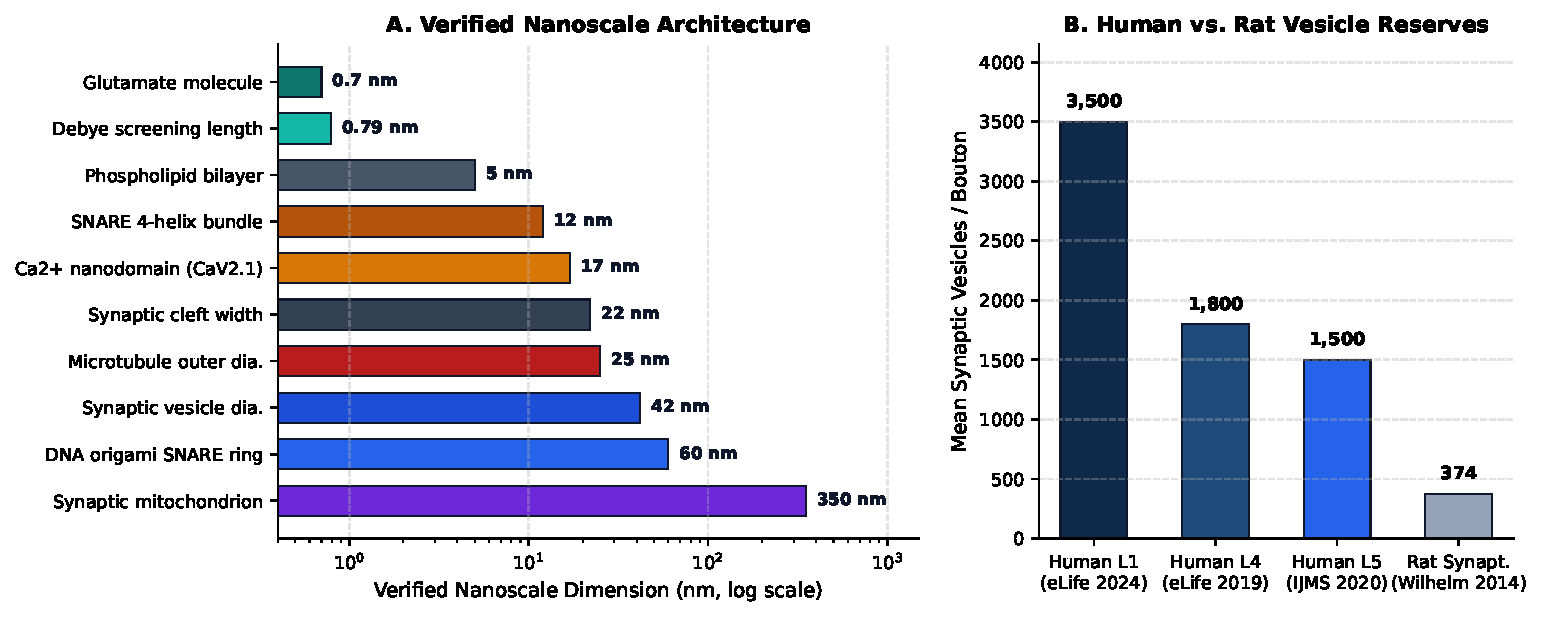
\includegraphics[width=0.95\textwidth]{../figures/fig1_nanoscale_architecture.pdf}
\caption{Verified nanoscale synaptic dimensions across three orders of magnitude (A) and human temporal neocortical Layer~1/4/5 vesicle reserves compared with the rat synaptosome baseline (B). Generated deterministically by \texttt{synapse-media}.}
\label{fig:arch}
\end{figure}

\section{Formal Verification in Lean~4.35.0, Adversarial Checks, and Statement Fidelity}

To eliminate floating-point artifacts and vacuous definitions in our discrete core, we formalized 24 elementary biophysical, discrete-dynamical, and $2\times 2$ integer determinant invariants in pure Lean~4.35.0 (\path{lean/Challenge.lean}, \path{lean/Solution.lean}) without Mathlib. In v1.4.0, we removed every unused hypothesis across all 24 theorems (strengthening \texttt{T02} to prove $0 < K_d^4 + K_d^4 \wedge 2 K_d^4 = K_d^4 + K_d^4$ and generalizing \texttt{T07} by dropping its unused $u_0 > 0$ guard), paired them with 27 concrete physiological non-vacuity witnesses (\path{lean/NonVacuity.lean}), 7 machine-checked sanity and sharpness checks (\path{lean/AdversarialChecks.lean}), an automated axiom audit (\path{lean/VerifyAxioms.lean}) drift-checked against \path{README.md}, an executable vector bridge (\path{lean/ExportVectors.lean} $\to$ \path{data/lean_engine_vectors.json}) tested against Python, TypeScript, and Rust, and an interactive browser Proof Blueprint DAG (\path{blueprint/index.html}). Related prior work applying Lean to quantitative science includes chemical physics formalization \cite{bobbin2024lean}, gene-regulatory network ODEs (\texttt{marpaia/grn-lean}), and SciLean scientific computing; our contribution differs by targeting zero-Mathlib, six-kernel replayable elementary synaptic invariants linked directly to a multi-language simulator.

\begin{theorem}[Hill $n=4$ Crossover \& Tsodyks--Markram STP Bounds]
In \path{lean/Solution.lean}, for exact natural-number concentrations $c, K_d \in \mathbb{N}$ with $K_d > 0$:
\begin{enumerate}
  \item $P_r(c) = \frac{c^4}{c^4 + K_d^4} \in [0,1)$, $0 < K_d^4 + K_d^4 \wedge 2 K_d^4 = K_d^4 + K_d^4$ ($P_r(K_d) = \frac{1}{2}$), and $c_1 < c_2 \implies P_r(c_1) < P_r(c_2)$ (axiom-free);
  \item Whenever $3c \le K_d$, $0 < c^4 + K_d^4$ and $82c^4 \le c^4 + K_d^4$ ($P_r \le \frac{1}{82} \approx 1.22\%$); doubling from $h = K_d/2 > 0$ to $2h = K_d$ multiplies $P_r$ by exactly $\frac{17}{2} = 8.5\times$;
  \item \emph{Sigmoidal crossover vs.\ linear sensor:} for $c > 0$, $c < K_d$ implies $\frac{c^4}{c^4 + K_d^4} < \frac{c}{c + K_d}$ (stronger sub-threshold noise suppression), whereas $c > K_d$ implies $\frac{c^4}{c^4 + K_d^4} > \frac{c}{c + K_d}$ (sharper supra-threshold saturation), with exact equality at $c = K_d$ (check \texttt{A06} in \path{AdversarialChecks.lean});
  \item \emph{Fixed-point Tsodyks--Markram STP:} for scale $S > 0$, $u \le S$, $u_0 \le S$, and $x \le S$, the discrete facilitation update $u^+ = u + \lfloor u_0(S-u)/S \rfloor$ and effective release $r = \lfloor u^+ x / S \rfloor$ satisfy $u \le u^+ \le S$, $r \le x$, and $x - r \le S$.
\end{enumerate}
\end{theorem}

\begin{theorem}[KCC2 Shunting \& NMDAR $\mathrm{Mg}^{2+}$ Coincidence Unblock]
In \path{lean/Solution.lean}, for integers $g_L, g_E, g_I > 0$ and reversal potentials $E_I \le E_L < E_E$:
\[
E_I \le \frac{g_L E_L + g_E E_E + g_I E_I}{g_L + g_E + g_I} < \frac{g_L E_L + g_E E_E}{g_L + g_E} \le E_E,
\]
with strictly positive denominators and nonzero excitatory drive $g_E(E_E - E_L) > 0$ certifying the pure-shunting ($E_I = E_L$) divisive ratio $(g_L + g_E)/(g_L + g_E + g_I)$. Moreover, for cleared-denominator Jahr--Stevens NMDAR unblock $B(V) = D/(D + M\cdot E(V))$ with $D, M > 0$ and $0 < E_{\mathrm{depol}} < E_{\mathrm{rest}}$ (monotonicity in the supplied positive exponential terms), both unblocked fractions lie strictly in $(0,1)$ and $B(V_{\mathrm{rest}}) < B(V_{\mathrm{depol}})$.
\end{theorem}

\begin{theorem}[Multi-Step Vesicle Conservation \& ATP Depletion Upper Bound]
In \path{lean/Solution.lean}, structural induction over any finite conservative cycling trace $\tau \in \mathrm{List}(\mathbb{N}^3)$ satisfying step-wise pool bounds (\path{ValidVesicleTrace}) proves total presynaptic vesicles are strictly conserved:
\[
(\mathrm{runVesicleTrace}\,p\,\tau).\mathrm{total} = p.\mathrm{total}.
\]
Under any strict local ATP deficit $D = (B_{\mathrm{leak}} + f\cdot C_{\mathrm{AP}}) - S_{\mathrm{ATP}} > 0$ starting from $A_0 > 0$, the clamped store drops strictly below $A_0$ for all $t > 0$ (\texttt{T14}) and reaches zero for every duration $t \ge \lfloor A_0 / D \rfloor + 1$ (\texttt{T15}, an \emph{upper bound} on hitting time; check \texttt{A07} proves that when $D \mid A_0$, depletion occurs strictly earlier at $t = A_0 / D$). Under the illustrative H3 40\,Hz model constants ($A_0 = 10^6$, $D = 334{,}000$), $\lfloor 10^6 / 334{,}000 \rfloor + 1 = 3$, certifying depletion by $t \ge 3\,$s.
\end{theorem}

\begin{table}[htbp]
\centering
\caption{Statement Fidelity Audit Summary (24 Lean~4.35.0 Lemmas + 7 Sanity/Sharpness Checks). Full table in \texttt{docs/statement-fidelity.md}.}
\label{tab:fidelity}
\footnotesize
\begin{tabularx}{\textwidth}{@{}>{\raggedright\arraybackslash}p{4.25cm}>{\raggedright\arraybackslash}p{4.25cm}>{\raggedright\arraybackslash}p{2.75cm}L@{}}
\toprule
\textbf{Lean Declarations} & \textbf{Formalized Claim} & \textbf{Anchor} & \textbf{Witnesses \& Axioms} \\
\midrule
\texttt{hill4\_*} (T01--T06), \texttt{tsodyks\_markram\_*} (T07) & Hill $n=4$ bounds, $1/82$ floor, $8.5\times$ gain, $n=4$ vs.\ $n=1$ crossover, STP unit bounds (0 unused hyps). & Dodge--Rahamimoff \cite{dodge1967calcium}; Tsodyks \cite{tsodyks1998dynamic} & 8 witnesses; \texttt{[]} (T03), \texttt{[propext]} (T06), \texttt{[propext, Quot.sound]}. \\
\texttt{ei\_*}, \texttt{shunting\_*}, \texttt{nmda\_mg\_*} (T08--T11) & Conductance divider bounds, KCC2 shunting attenuation, NMDAR unblock in $(0,1)$ \& monotone in $E$. & Conductance divider; Jahr--Stevens \cite{jahr1990nmda} & 4 witnesses ($1,3,4\,$nS; $-70$ vs.\ $+20\,$mV); \texttt{[propext, Quot.sound]}. \\
\texttt{vesicle\_pool\_*}, \texttt{atp\_*}, \texttt{resting\_leak\_*}, \texttt{kinesin\_*} (T12--T17) & Single/multi-step vesicle induction, clamped ATP drop, hitting-time upper bound ($t\ge 3\,$s), leak bounds, $125{,}000\,$ATP/mm. & Rollenhagen \cite{rollenhagen2024l1}; Rangaraju \cite{rangaraju2014atp}; Pulido \cite{pulido2021resting} & 8 witnesses (Rat 374, Human L1 3,500 3-step, H3 $t=3\,$s); \texttt{[propext, Quot.sound]}. \\
\texttt{snare\_*} (T18--T19), \texttt{resi\_*} (T20--T21) & Syt1/copy-number fusion barrier monotonicity; RESI $1/(N K)$ variance \& imager duty cycle. & Xu \cite{xu2016dnaorigami}; Reinhardt \cite{reinhardt2023resi} & 4 witnesses; \texttt{[]} on duty cycle (T21), \texttt{[propext, Quot.sound]}. \\
\texttt{factorized\_*}, \texttt{correlated\_*}, \texttt{diagonal\_excess\_*} (T22--T24) & Product $2\times 2$ integer tables have $0$ det.; diagonal dominance/excess gives $>0$ (also generic aliases). & Elementary $2\times 2$ matrix algebra & 3 witnesses; \texttt{[propext]} (T23), \texttt{[propext, Quot.sound]}. \\
\texttt{AdversarialChecks.*} (A01--A07) & Negation/sharpness checks for $K_d>0$, $g_E>0$, $A_0>0$, $C_{\mathrm{AP}}\le B_{\mathrm{leak}}$, $c=K_d$, $(40,10;10,40)$, \& $D \mid A_0$. & Playbook v1.3 Item 12 & 7 sanity \& sharpness checks (\texttt{A01}--\texttt{A07}). \\
\bottomrule
\end{tabularx}
\end{table}

\textbf{Multi-Kernel Verification Result.} Building \texttt{lean/} with \texttt{lake build --wfail} succeeded with zero warnings and zero errors. All 24 theorems depend on zero \texttt{Classical.choice}, zero \texttt{sorryAx}, zero \texttt{Lean.ofReduceBool}, and zero \texttt{\_native} axioms (two theorems use \emph{no axioms at all} and two use only \texttt{propext}), strictly enforced by \path{lean/comparator.json} (\texttt{permitted\_axioms: ["propext", "Quot.sound"]}), \path{scripts/check_readme_axioms.py}, and repository CI. Repository Ubuntu CI (\path{.github/workflows/ci.yml}) replays \texttt{lake comparator --paranoid} across six independent kernels (\texttt{lean}, \texttt{leanchecker-paranoid}, \texttt{lean4lean}, \texttt{nanoda}, \texttt{con-leche}, and \texttt{con-ron}; note that standalone \texttt{nanoda\_bin} receives \texttt{Classical.choice} only in its transitive \texttt{Init} export config, while all 24 theorem axiom footprints are strictly forbidden from using \texttt{Classical.choice}), checks \texttt{NonVacuity} and \texttt{AdversarialChecks} via \texttt{leanchecker}, and verifies \texttt{ExportVectors.lean} parity against \path{data/lean_engine_vectors.json}.

\section{Electrophysiology, SNARE Thermodynamics, Bioenergetics, and Metrology}

Figure~\ref{fig:elec} presents our verified electrophysiological stack: stationary linearized-buffer $\mathrm{Ca}^{2+}$ nanodomain decay ($d \le 17\,$nm, modeled after Naraghi--Neher \cite{naraghi1997buffered}), Hill $n=4$ release probability \cite{dodge1967calcium} with kernel-checked anchors, 4D Hodgkin--Huxley RK4 action potential integration \cite{hodgkin1952quantitative} (explicitly tagged \texttt{numerical\_approximation}), and Jahr--Stevens NMDAR $\mathrm{Mg}^{2+}$ voltage unblock \cite{jahr1990nmda}.

\begin{figure}[htbp]
\centering
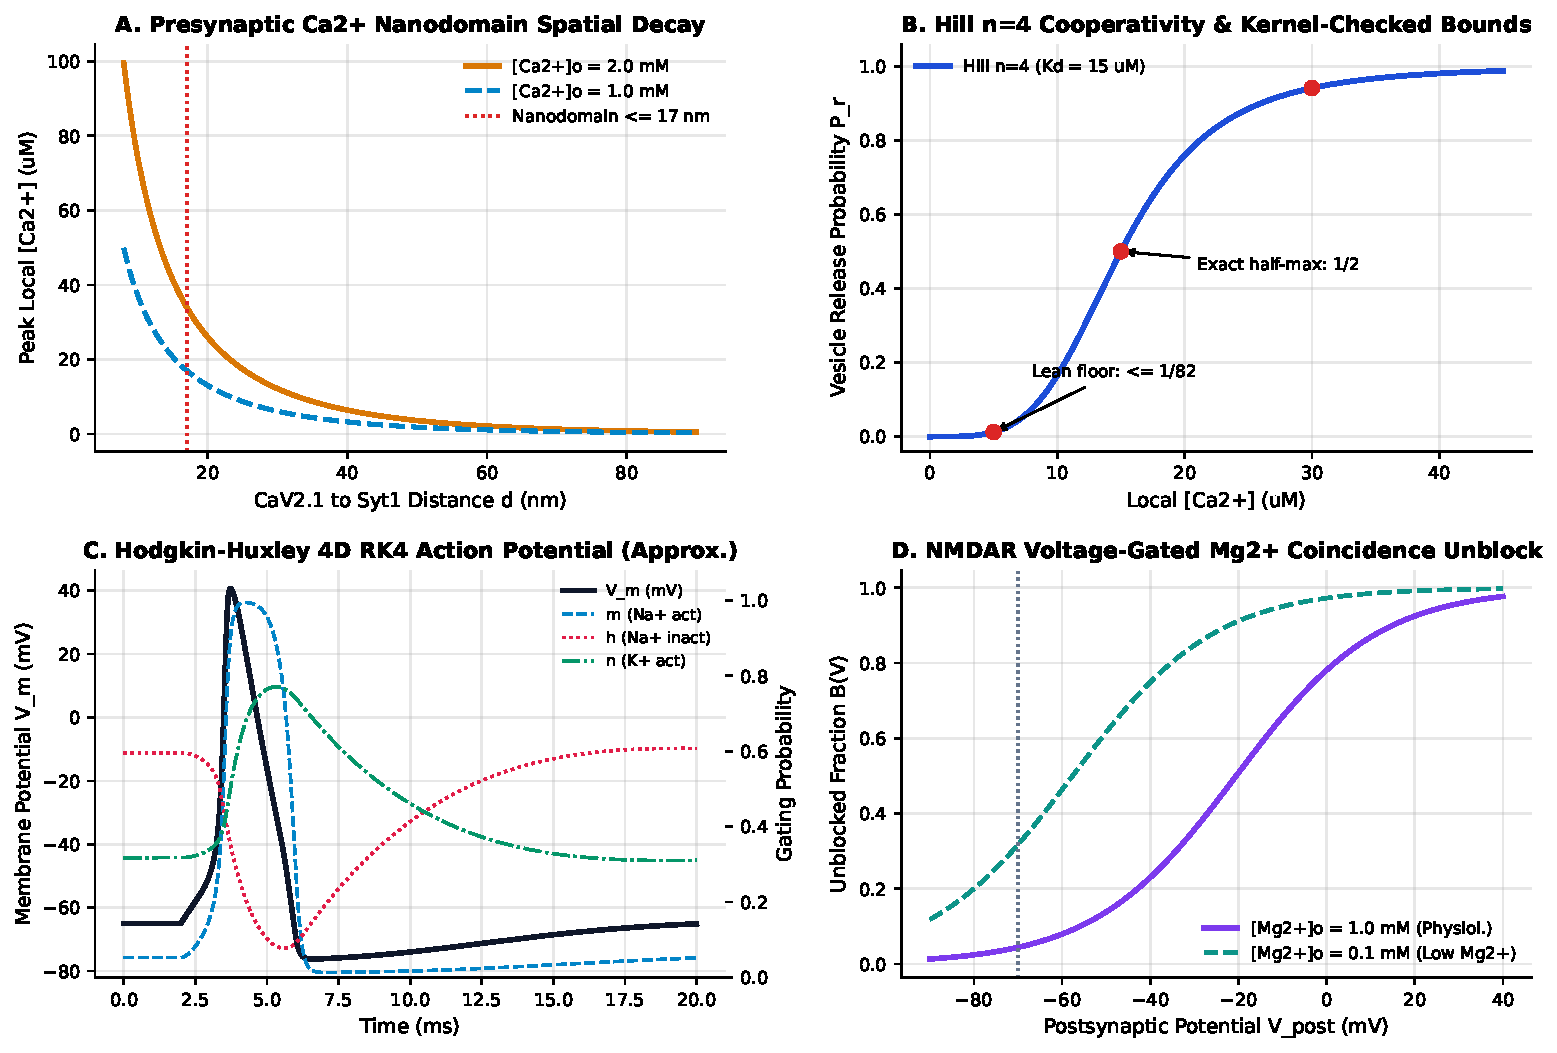
\includegraphics[width=0.95\textwidth]{../figures/fig2_electrophysiology_hodgkin_huxley.pdf}
\caption{Quantitative electrophysiology generated from our verified 50-digit oracle and RK4 solver: (A) presynaptic $\mathrm{Ca}^{2+}$ nanodomain decay, (B) Hill $n=4$ release curve with Lean-proved bounds, (C) 4D Hodgkin--Huxley RK4 action potential and $(m,h,n)$ gating, and (D) NMDAR $\mathrm{Mg}^{2+}$ voltage-gated coincidence unblock.}
\label{fig:elec}
\end{figure}

At the organic-biochemistry layer, classic lipidomics of cholinergic synaptic vesicles from the marine ray \emph{Narcine brasiliensis} electric organ reported an asymmetric high-curvature lipidome ($33.3\%$ cholesterol, $32.3\%$ PC, $20.5\%$ PE, $6.1\%$ PS, $3.0\%$ sphingomyelin, enriched in DHA~22:6 \cite{deutsch1981lipids}; note the non-human species and cholinergic preparation). Recent native synaptic vesicle cryo-EM studies resolved cholesterol decorating the V-ATPase $V_0$ rotor and ATP-hydrolysis/loading-coupled $V_1$ dissociation in rat brain vesicles \cite{coupland2024vatpase}, alongside the V-ATPase--synaptophysin structural interface and vesicle copy-number topography in mouse vesicles \cite{wang2024vatpase}. Clostridial zinc metalloproteases (BoNT/A--G, TeNT) selectively cleave unassembled SNARE proteins \cite{dong2019neurotoxins}. Figure~\ref{fig:chem} shows the SNAREpin free-energy reaction coordinate switching from Complexin-arrested ($0\,\mathrm{Ca}^{2+}$) to sub-millisecond synchronous fusion ($5\,\mathrm{Ca}^{2+}$ on Syt1 C2A/C2B), logarithmic ATP cost scaling (including $125{,}000\,$ATP/mm for kinesin-1), and RESI $1/\sqrt{N\cdot K}$ localization scaling \cite{reinhardt2023resi} enabling DNA-origami SNARE stoichiometry rings \cite{xu2016dnaorigami} to be resolved below $1\,$nm.

\begin{figure}[htbp]
\centering
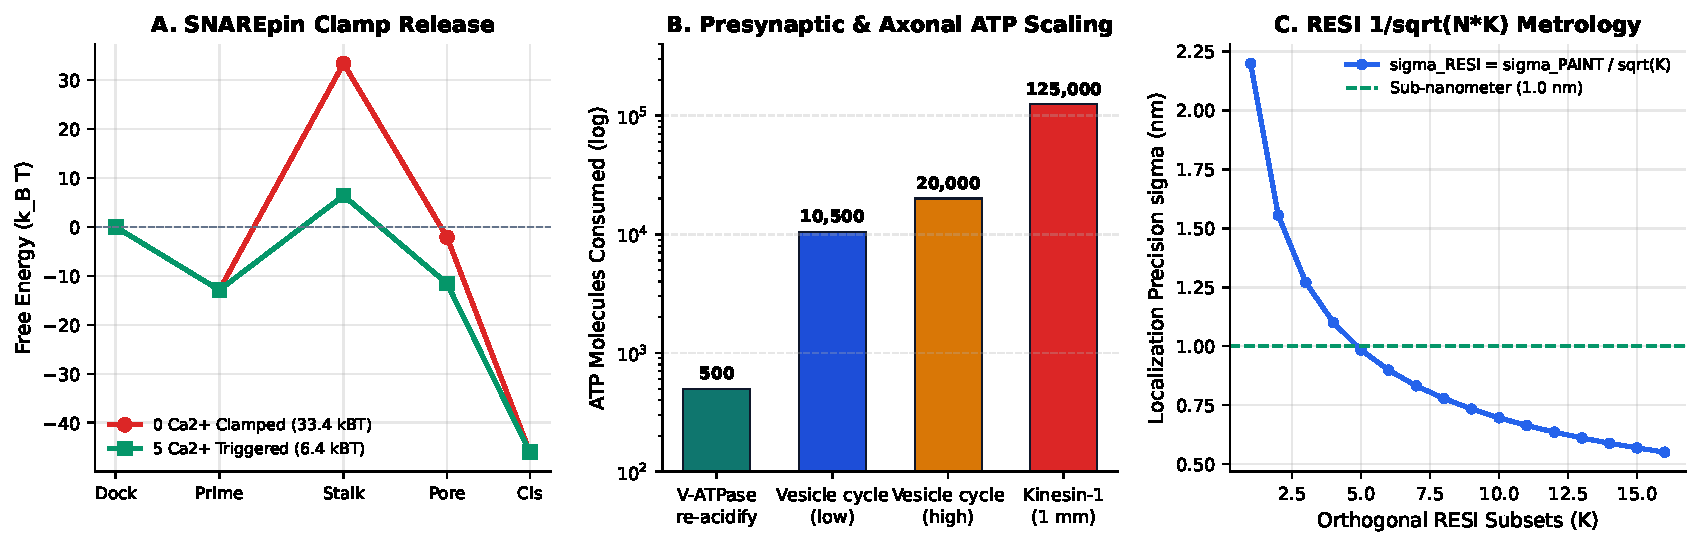
\includegraphics[width=0.96\textwidth]{../figures/fig3_snare_bioenergetics_metrology.pdf}
\caption{(A) SNAREpin free-energy coordinate ($0$ vs.\ $5\,\mathrm{Ca}^{2+}$ bound to Syt1), (B) log-scale presynaptic and axonal ATP expenditure, and (C) DNA-PAINT to RESI sub-nanometer precision scaling.}
\label{fig:chem}
\end{figure}

\section{Pre-Registered 30-Seed Monte Carlo Results and Honest Failure of H3}

Before executing any stochastic simulation, we committed \path{PREREGISTRATION.md} at root SHA \texttt{a1919f2} fixing the directional hypotheses, seed blocks $S=\{1000,\dots,1029\}$ ($N=30$ per arm) and null control $S_{\mathrm{null}}=\{2000,\dots,2029\}$, 10,000-permutation tests, 10,000-resample 95\% bootstrap CIs, and Holm--Bonferroni correction. In transparent audit disclosure, \path{PREREGISTRATION.md} fixed the hypotheses, seeds, and statistical plan prior to running the code, whereas the specific illustrative bioenergetic rate constants in Rust/TypeScript ($10^6$ free ATP pool, $950{,}000\,$ATP/s mitochondrial synthesis, $280{,}000\,$ATP/s glycolysis, $4{,}000\,$ATP/s resting leak---compared with $\sim 3{,}100\,$ATP/s measured in cultured rat hippocampal boutons by Pulido \& Ryan \cite{pulido2021resting}---and $32{,}000\,$ATP/AP) were instantiated when the simulation engine was written. Consequently, H1--H4 test deterministic fixed-parameter properties of this specific biophysical simulator rather than new wet-lab measurements. All computations executed deterministically in Rust (\texttt{ChaCha8Rng}) and were analyzed in Python (\path{synapse-stats}), accompanied by Croissant~1.0 dataset metadata (\path{croissant.json}).

\begin{figure}[htbp]
\centering
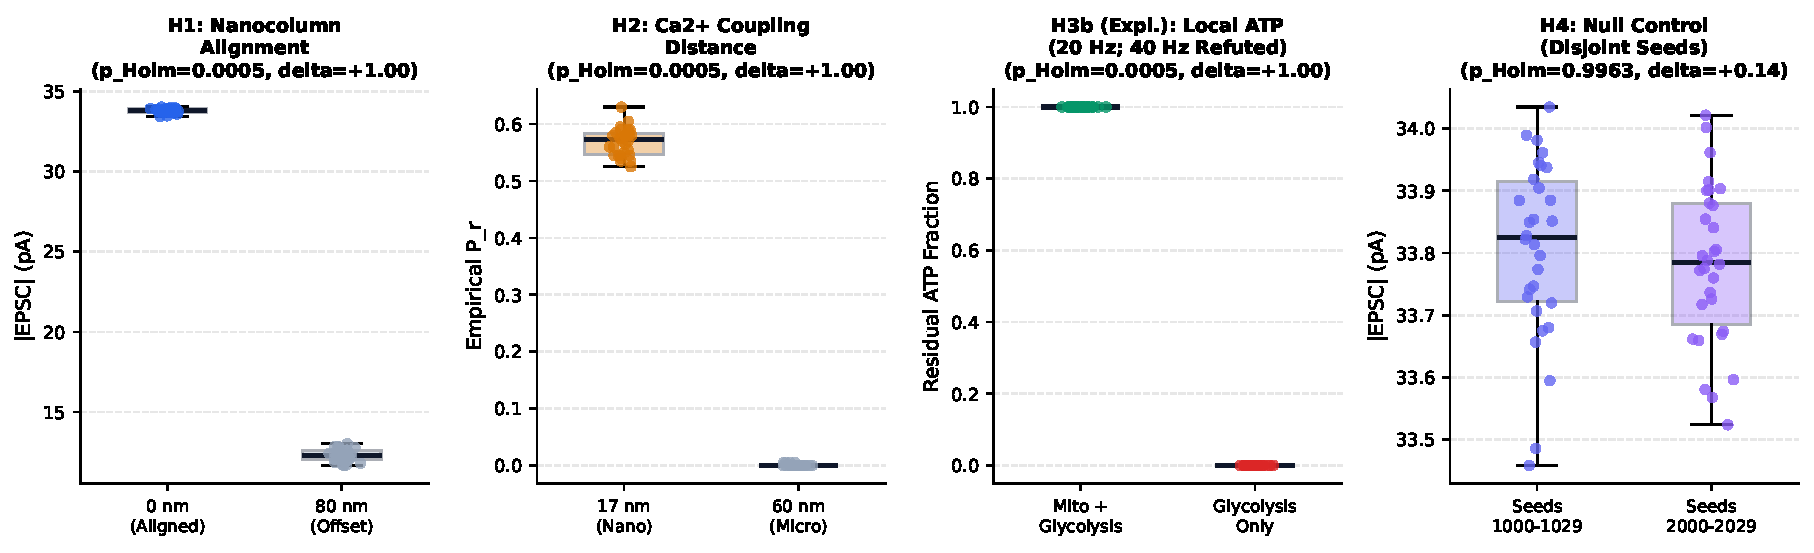
\includegraphics[width=0.96\textwidth]{../figures/fig4_preregistered_monte_carlo.pdf}
\caption{30-seed Monte Carlo distributions with individual seed points, medians, Holm--Bonferroni adjusted permutation $p$-values, and Cliff's $\delta$ across H1, H2, exploratory H3b (20\,Hz; pre-registered 40\,Hz H3 failed in simulation as logged in \texttt{DEVIATIONS.md}), and the disjoint-seed null control H4.}
\label{fig:mc}
\end{figure}

\noindent\textbf{Key Simulator Outcomes (Figure~\ref{fig:mc}):}\par\nopagebreak
\begin{itemize}
  \item \textbf{H1 (Confirmed in Simulation):} Presynaptic release alignment with postsynaptic AMPAR nanocolumns ($0$ vs.\ $80\,$nm offset \cite{tang2016nanocolumn}) raises mean peak $|\text{EPSC}|$ from $12.28$ to $33.81\,$pA ($\Delta = +21.53\,$pA, 95\% CI $[21.42, 21.63]$, $\delta = +1.00$, $p_{\mathrm{Holm}} = 0.0005$).
  \item \textbf{H2 (Confirmed in Simulation):} Tight $17\,$nm $\mathrm{Ca}^{2+}$ nanodomain coupling increases empirical release probability $\hat{P}_r$ from $0.0007$ ($60\,$nm microdomain) to $0.569$ ($\Delta = +0.568$, 95\% CI $[0.560, 0.577]$, $\delta = +1.00$, $p_{\mathrm{Holm}} = 0.0005$).
  \item \textbf{H3 (Pre-Registered at 40\,Hz — Failed in Simulation):} Our pre-registered prediction stated that mitochondria would retain $>90\%$ ATP at $40\,$Hz over $60\,$s. In execution, mean ATP burn of $1{,}284{,}000\,$ATP/s ($4{,}000$ resting leak plus $40 \times 32{,}000$ firing cost) exceeded \emph{both} glycolysis ($280{,}000\,$ATP/s) and mitochondrial OxPhos ($950{,}000\,$ATP/s, critical frequency $f_{\mathrm{crit,mito}} = 29.5625\,$Hz), driving both arms to $0.0$ ($p_{\mathrm{Holm}}=1.0$, $\delta=0.0$; Lean~4 Theorem~\texttt{T15} gives the depletion upper bound $t \ge 3\,$s under mean rates). Rather than silently altering H3, we report the failure verbatim and log a separate post-hoc exploratory arm \texttt{H3b} at $20\,$Hz in \path{DEVIATIONS.md}, where mitochondria sustain $100\%$ ATP while glycolysis depletes to $0\%$ ($p_{\mathrm{Holm}}=0.0005$, $\delta=+1.00$).
  \item \textbf{H4 (Null Control Passed):} Disjoint seed cohorts ($1000\text{--}1029$ vs.\ $2000\text{--}2029$) show no significant difference ($\Delta = +0.024\,$pA, 95\% CI $[-0.045, +0.091]$, $p_{\mathrm{Holm}} = 0.9963$), confirming absence of RNG bias.
\end{itemize}

\section{Limitations, Threats to Validity, Reproducibility, and Disclosures}

\textbf{Limitations.} (1) Our active-zone diffusion model uses a stationary Naraghi--Neher linearized approximation \cite{naraghi1997buffered} rather than meshed 3D Brownian MCell4/BioNetGen particle simulation; (2) Hodgkin--Huxley RK4 and Monte Carlo sweeps are \texttt{numerical\_approximation} rather than formally verified Lean interval ODE enclosures; (3) the bioenergetic constants in H3/H3b are illustrative model parameters instantiated after \path{PREREGISTRATION.md} was committed, and the vesicle lipidome derives from \emph{Narcine brasiliensis} rather than human cortex; (4) deterministic 2D/3D workbench schematics are educational models, not atomic PDB/EMDB coordinate renders.

\textbf{Reproducibility and Cryptographic Provenance.} Every theorem, test, benchmark, figure, video, and PDF regenerates cleanly from a fresh clone via pinned lockfiles (\path{lean-toolchain}, \path{Cargo.lock}, \path{uv.lock}, \path{package-lock.json}), a digest-pinned \path{Dockerfile}, and \texttt{just reproduce}. All five Lean~4.35.0 proof modules carry \texttt{module} headers and pass \texttt{lake comparator --paranoid} across six independent kernels in public repository Ubuntu CI with zero \texttt{Classical.choice}. Cross-language differential testing verifies $1{,}000$ random inputs plus exported Lean vectors (\path{data/lean_engine_vectors.json}) across TypeScript, Rust, and 50-digit Python (with \texttt{NaN}/\texttt{Inf} and domain boundary guards) with zero mismatches; targeted mutation testing (\path{scripts/mutation_audit.py}) enforces an unmutated \texttt{rc=0} baseline control and strictly kills $6/6$ core biophysical mutants (\texttt{rc=1}); live Crossref citation auditing verifies $28$ DOI-bearing entries for HTTP~200, normalized title match, first-author surname, year, and retraction status (zero retractions; one publisher correction on Wang~2024) plus $1$ non-DOI entry (\texttt{chalmers1995facing}, total $29$, \path{docs/citation-audit.json}). Permanent archival is recorded at CERN Zenodo (Concept DOI \href{https://doi.org/10.5281/zenodo.24477927}{10.5281/zenodo.24477927}, resolving to the latest release; prior v1.3.0 DOI \href{https://doi.org/10.5281/zenodo.24548051}{10.5281/zenodo.24548051}; prior v1.2.0 DOI \href{https://doi.org/10.5281/zenodo.24484350}{10.5281/zenodo.24484350}) and Software Heritage (prior v1.2.0 snapshot \nolinkurl{swh:1:snp:8ef70f745fae4f91f040720b28e21560c73deffc}), sealed by root \path{MANIFEST.sha256}, DigiCert RFC~3161 timestamp, GitHub SLSA release attestations, \path{ERRATA.md} (with explicit Withdrawal \& Retraction Policy), and \path{HARDENING_LOG.md}. Live workbench: \url{https://0thernes.github.io/human-synapse-bouton-lab/}; live Lean Proof Blueprint: \url{https://0thernes.github.io/human-synapse-bouton-lab/blueprint/}.

\textbf{AI-Contribution Statement (CRediT) and Conflict of Interest.} Author: Alexander Stephen Donahue (ORCID \href{https://orcid.org/0009-0006-8168-9648}{0009-0006-8168-9648}), Independent Researcher. Human CRediT roles: Conceptualization; Methodology; Formal analysis (definition design, positive-domain tightening, statement-fidelity audit); Validation; Writing -- review \& editing. AI tools used: Antigravity (Google DeepMind) assisted with multi-language software refactoring, Lean~4 proof drafting, and LaTeX typesetting (full disclosure in \path{docs/AI_DISCLOSURE.md}). All formal proofs are independently certified by the Lean~4.35.0 kernel and external checkers; no AI system is listed as an author. The author takes full responsibility for all content. Conflict of Interest: none declared; no external funding, employer, or corporate entity.

\bibliographystyle{plain}
\bibliography{../references}

\end{document}
